\chapter{Ordenació}
\index{ordenació}

El problema de l'\key{ordenació}
és un problema fonamental del disseny d'algorismes.
Molts algorismes eficients
fan servir l'ordenació com a subrutina,
perquè sovint és més fàcil de processar
dades si els elements estan ordenats.

Per exemple, el problema de ``té un vector dos elements iguals?'' és
fàcil de resoldre mitjançant l'ordenació.  Si el vector conté dos
elements iguals, després d'ordenar-los estaran l'un al costat de
l'altre, de manera que és fàcil trobar-los.  El problema ``quin és
l'element més freqüent d'un vector?'' es pot resoldre de la mateixa
manera.

Hi ha molts algorismes per ordenar, i aquests són
també bons exemples de com aplicar
diferents tècniques del disseny d'algorismes.
Els algorismes d'ordenació general eficients
treballar en temps $O(n \log n)$,
i molts algorismes que utilitzen l'ordenació
com a subrutina tenen també aquesta complexitat temporal.

\section{Teoria de l'ordenació}

El problema bàsic de l'ordenació és el següent:
\begin{framed}
\noindent
Donat un vector que conté $n$ elements,
ordena els elements en ordre creixent.
\end{framed}
\noindent
Per exemple, el vector
\begin{center}
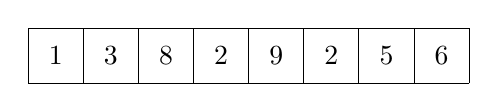
\begin{tikzpicture}[scale=0.7]
\draw (0,0) grid (8,1);
\node at (0.5,0.5) {$1$};
\node at (1.5,0.5) {$3$};
\node at (2.5,0.5) {$8$};
\node at (3.5,0.5) {$2$};
\node at (4.5,0.5) {$9$};
\node at (5.5,0.5) {$2$};
\node at (6.5,0.5) {$5$};
\node at (7.5,0.5) {$6$};
\end{tikzpicture}
\end{center}
queda de la manera següent després d'ordenar-lo:
\begin{center}
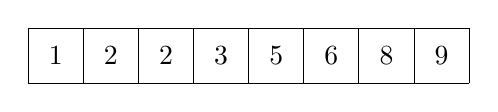
\begin{tikzpicture}[scale=0.7]
\draw (0,0) grid (8,1);
\node at (0.5,0.5) {$1$};
\node at (1.5,0.5) {$2$};
\node at (2.5,0.5) {$2$};
\node at (3.5,0.5) {$3$};
\node at (4.5,0.5) {$5$};
\node at (5.5,0.5) {$6$};
\node at (6.5,0.5) {$8$};
\node at (7.5,0.5) {$9$};
\end{tikzpicture}
\end{center}

\subsubsection{Algorismes $O(n^2)$}

\index{ordenació amb bombolla}

Alguns algorismes senzills per ordenar un vector
treballen en temps $O(n^2)$.
Aquests algorismes són curts i generalment
consten de dos bucles niats.
Un algorisme famós amb complexitat $O(n^2)$
és \key{l'ordenació amb bombolla} (\key{bubble sort})
on els elements del vector es mouen
com si fossin ``bombolles''.

L'ordenació amb bombolla consta de $n$ rondes.
A cada ronda, l'algorisme itera
els elements del vector.
Sempre que es troben dos elements consecutius
que no estan en ordre correcte,
l'algorisme els intercanvia.
L'algorisme es pot implementar de la següent manera:
\begin{lstlisting}
for (int i = 0; i < n; i++) {
    for (int j = 0; j < n-1; j++) {
        if (v[j] > v[j+1]) {
            swap(v[j],v[j+1]);
        }
    }
}
\end{lstlisting}

Després de la primera ronda de l'algorisme,
l'element més gran estarà en la posició correcta,
i en general, després de $k$ rondes, els $k$ elements
més grans estaran en les posicions correctes.
Així, després de $n$ rondes, el vector quedarà
ordenat.

Per exemple, en el vector

\begin{center}
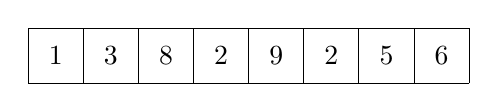
\begin{tikzpicture}[scale=0.7]
\draw (0,0) grid (8,1);

\node at (0.5,0.5) {$1$};
\node at (1.5,0.5) {$3$};
\node at (2.5,0.5) {$8$};
\node at (3.5,0.5) {$2$};
\node at (4.5,0.5) {$9$};
\node at (5.5,0.5) {$2$};
\node at (6.5,0.5) {$5$};
\node at (7.5,0.5) {$6$};
\end{tikzpicture}
\end{center}

\noindent
la primera ronda d'ordenació amb bombolla intercanvia els
elements com segueix:

\begin{center}
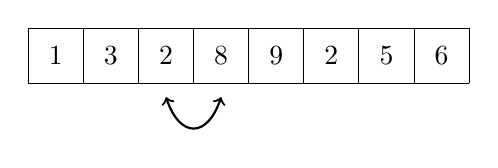
\begin{tikzpicture}[scale=0.7]
\draw (0,0) grid (8,1);
\node at (0.5,0.5) {$1$};
\node at (1.5,0.5) {$3$};
\node at (2.5,0.5) {$2$};
\node at (3.5,0.5) {$8$};
\node at (4.5,0.5) {$9$};
\node at (5.5,0.5) {$2$};
\node at (6.5,0.5) {$5$};
\node at (7.5,0.5) {$6$};

\draw[thick,<->] (3.5,-0.25) .. controls (3.25,-1.00) and (2.75,-1.00) .. (2.5,-0.25);
\end{tikzpicture}
\end{center}

\begin{center}
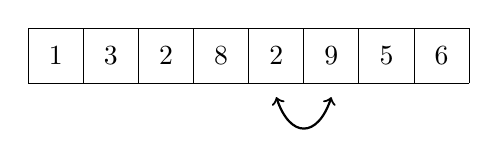
\begin{tikzpicture}[scale=0.7]
\draw (0,0) grid (8,1);
\node at (0.5,0.5) {$1$};
\node at (1.5,0.5) {$3$};
\node at (2.5,0.5) {$2$};
\node at (3.5,0.5) {$8$};
\node at (4.5,0.5) {$2$};
\node at (5.5,0.5) {$9$};
\node at (6.5,0.5) {$5$};
\node at (7.5,0.5) {$6$};

\draw[thick,<->] (5.5,-0.25) .. controls (5.25,-1.00) and (4.75,-1.00) .. (4.5,-0.25);
\end{tikzpicture}
\end{center}

\begin{center}
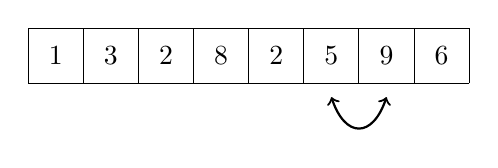
\begin{tikzpicture}[scale=0.7]
\draw (0,0) grid (8,1);
\node at (0.5,0.5) {$1$};
\node at (1.5,0.5) {$3$};
\node at (2.5,0.5) {$2$};
\node at (3.5,0.5) {$8$};
\node at (4.5,0.5) {$2$};
\node at (5.5,0.5) {$5$};
\node at (6.5,0.5) {$9$};
\node at (7.5,0.5) {$6$};

\draw[thick,<->] (6.5,-0.25) .. controls (6.25,-1.00) and (5.75,-1.00) .. (5.5,-0.25);
\end{tikzpicture}
\end{center}

\begin{center}
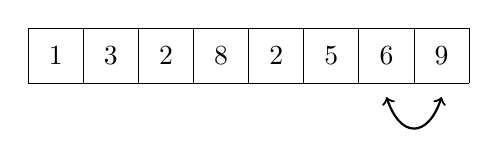
\begin{tikzpicture}[scale=0.7]
\draw (0,0) grid (8,1);
\node at (0.5,0.5) {$1$};
\node at (1.5,0.5) {$3$};
\node at (2.5,0.5) {$2$};
\node at (3.5,0.5) {$8$};
\node at (4.5,0.5) {$2$};
\node at (5.5,0.5) {$5$};
\node at (6.5,0.5) {$6$};
\node at (7.5,0.5) {$9$};

\draw[thick,<->] (7.5,-0.25) .. controls (7.25,-1.00) and (6.75,-1.00) .. (6.5,-0.25);
\end{tikzpicture}
\end{center}

\subsubsection{Inversions}

\index{inversió}

L'ordenació amb bombolla és un exemple
d'algorisme d'ordenació que sempre intercanvia
elements \emph{consecutius} del vector.
La complexitat temporal d'aquest algorisme
és $O(n^2)$, donat que aquest és el nombre de
comparacions que es fan. (I, en el pitjor cas, és
el nombre de swaps).

Un concepte útil a l'hora d'analitzar l'ordenació
algorismes és el concepte d'\key{inversió}, que són
els parells d'elements situats en l'ordre incorrecte, és
a dir, els parells
$(\texttt{v}[a],\texttt{v}[b])$ tal que
$a<b$ i $\texttt{v}[a]>\texttt{v}[b]$.
Per exemple, el vector
\begin{center}
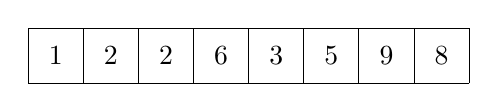
\begin{tikzpicture}[scale=0.7]
\draw (0,0) grid (8,1);
\node at (0.5,0.5) {$1$};
\node at (1.5,0.5) {$2$};
\node at (2.5,0.5) {$2$};
\node at (3.5,0.5) {$6$};
\node at (4.5,0.5) {$3$};
\node at (5.5,0.5) {$5$};
\node at (6.5,0.5) {$9$};
\node at (7.5,0.5) {$8$};
\end{tikzpicture}
\end{center}
té tres inversions: $(6,3)$, $(6,5)$ i $(9,8)$.
El nombre d'inversions indica
quanta feina és necessària per a ordenar el vector.
Un vector està completament ordenat quan
no hi ha inversions.
D'altra banda, si tots els elements del vector
estan en ordre invers,
el nombre d'inversions és el més gran possible:
\[1+2+\cdots+(n-1)=\frac{n(n-1)}{2} = O(n^2)\]

Intercanviar un parell d'elements consecutius en
ordre incorrecte elimina exactament una inversió
del vector.
Per tant, si un algorisme d'ordenació només
intercanvia elements consecutius, cada intercanvi elimina
com a màxim una inversió i la complexitat temporal
de l'algorisme és almenys $O(n^2)$.

\subsubsection{Algorismes $O(n \log n)$}

\index{merge sort}

És possible ordenar un vector de manera eficient
en temps $O(n \log n)$ fent servir algorismes
que no es limiten a intercanviar elements consecutius.
Un d'aquests algorismes és \key{merge sort}\footnote{Segons \cite{knu983},
el merge sort va ser inventat per J. von Neumann el 1945.},
que es basa en la recursivitat.

El merge sort ordena un subvector \texttt{v}$[a \ldots b]$ de la següent manera:

\begin{enumerate}
\item Si $a=b$, no feu res, perquè el subvector ja està ordenat.
\item Calcula la posició de l'element central: $k=\lfloor (a+b)/2 \rfloor$.
\item Ordena recursivament el subvector \texttt{v}$[a \ldots k]$.
\item Ordena recursivament el subvector \texttt{v}$[k+1 \ldots b]$.
\item Fusiona (\emph{merge}) els subvectors ordenats \texttt{v}$[a \ldots k]$ i
\texttt{v}$[k+1 \ldots b]$
en un subvector ordenat \texttt{v}$[a \ldots b]$.
\end{enumerate}

El merge sort és un algorisme eficient, perquè cada pas
redueix a la meitat la mida del subvector.
La recursivitat consisteix en $O(\log n)$ nivells,
i cada nivell triga temps $O(n)$.
És possible fusionar i ordenar els subvectors
\texttt{v}$[a \ldots k]$ i \texttt{v}$[k+1 \ldots b]$ en
temps lineal perquè ja estan ordenats.

Per exemple, considerem el vector següent:
\begin{center}
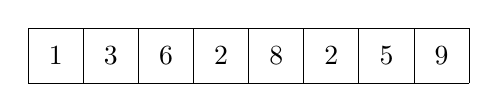
\begin{tikzpicture}[scale=0.7]
\draw (0,0) grid (8,1);
\node at (0.5,0.5) {$1$};
\node at (1.5,0.5) {$3$};
\node at (2.5,0.5) {$6$};
\node at (3.5,0.5) {$2$};
\node at (4.5,0.5) {$8$};
\node at (5.5,0.5) {$2$};
\node at (6.5,0.5) {$5$};
\node at (7.5,0.5) {$9$};
\end{tikzpicture}
\end{center}

Dividim el vector en dos subvectors:
\begin{center}
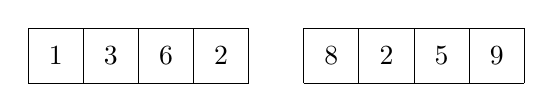
\begin{tikzpicture}[scale=0.7]
\draw (0,0) grid (4,1);
\draw (5,0) grid (9,1);

\node at (0.5,0.5) {$1$};
\node at (1.5,0.5) {$3$};
\node at (2.5,0.5) {$6$};
\node at (3.5,0.5) {$2$};

\node at (5.5,0.5) {$8$};
\node at (6.5,0.5) {$2$};
\node at (7.5,0.5) {$5$};
\node at (8.5,0.5) {$9$};
\end{tikzpicture}
\end{center}

Ordenem els subvectors de manera recursiva:
\begin{center}
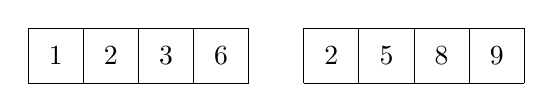
\begin{tikzpicture}[scale=0.7]
\draw (0,0) grid (4,1);
\draw (5,0) grid (9,1);

\node at (0.5,0.5) {$1$};
\node at (1.5,0.5) {$2$};
\node at (2.5,0.5) {$3$};
\node at (3.5,0.5) {$6$};

\node at (5.5,0.5) {$2$};
\node at (6.5,0.5) {$5$};
\node at (7.5,0.5) {$8$};
\node at (8.5,0.5) {$9$};
\end{tikzpicture}
\end{center}

Finalment, l'algorisme fusiona els subvectors
ordenats i crea el vector final:
\begin{center}
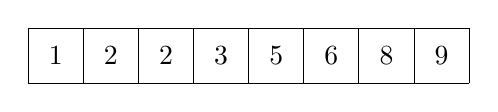
\begin{tikzpicture}[scale=0.7]
\draw (0,0) grid (8,1);
\node at (0.5,0.5) {$1$};
\node at (1.5,0.5) {$2$};
\node at (2.5,0.5) {$2$};
\node at (3.5,0.5) {$3$};
\node at (4.5,0.5) {$5$};
\node at (5.5,0.5) {$6$};
\node at (6.5,0.5) {$8$};
\node at (7.5,0.5) {$9$};
\end{tikzpicture}
\end{center}

\subsubsection{Límit inferior per l'ordenació}

És possible ordenar més ràpidament que en temps $O(n \log n)$?
Resulta que això \emph{no} és possible
quan fem servir algorismes d'ordenació
que es basen en comparar els elements d'un vector.

Aquest límit inferior $O(n \log n)$ es demostra si hom
considera l'ordenació com un procés on cada comparació
de dos elements proporciona més informació sobre el
contingut del vector original. El procés crea el següent arbre:

\begin{center}
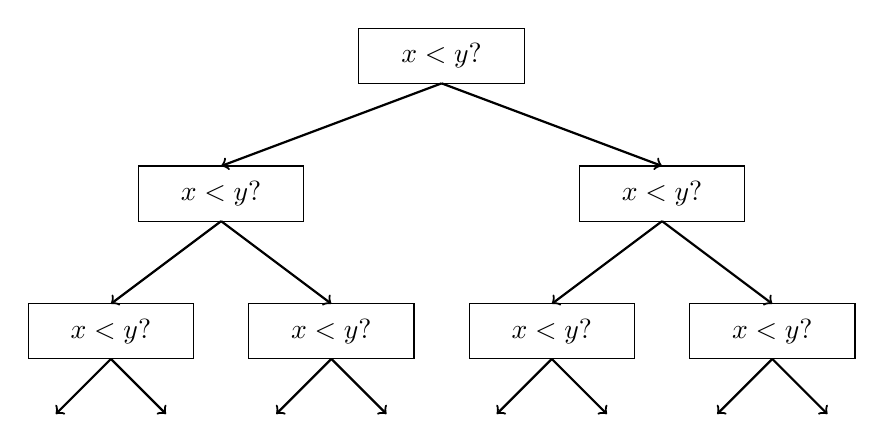
\begin{tikzpicture}[scale=0.7]
\draw (0,0) rectangle (3,1);
\node at (1.5,0.5) {$x < y?$};

\draw[thick,->] (1.5,0) -- (-2.5,-1.5);
\draw[thick,->] (1.5,0) -- (5.5,-1.5);

\draw (-4,-2.5) rectangle (-1,-1.5);
\draw (4,-2.5) rectangle (7,-1.5);
\node at (-2.5,-2) {$x < y?$};
\node at (5.5,-2) {$x < y?$};

\draw[thick,->] (-2.5,-2.5) -- (-4.5,-4);
\draw[thick,->] (-2.5,-2.5) -- (-0.5,-4);
\draw[thick,->] (5.5,-2.5) -- (3.5,-4);
\draw[thick,->] (5.5,-2.5) -- (7.5,-4);

\draw (-6,-5) rectangle (-3,-4);
\draw (-2,-5) rectangle (1,-4);
\draw (2,-5) rectangle (5,-4);
\draw (6,-5) rectangle (9,-4);
\node at (-4.5,-4.5) {$x < y?$};
\node at (-0.5,-4.5) {$x < y?$};
\node at (3.5,-4.5) {$x < y?$};
\node at (7.5,-4.5) {$x < y?$};

\draw[thick,->] (-4.5,-5) -- (-5.5,-6);
\draw[thick,->] (-4.5,-5) -- (-3.5,-6);
\draw[thick,->] (-0.5,-5) -- (0.5,-6);
\draw[thick,->] (-0.5,-5) -- (-1.5,-6);
\draw[thick,->] (3.5,-5) -- (2.5,-6);
\draw[thick,->] (3.5,-5) -- (4.5,-6);
\draw[thick,->] (7.5,-5) -- (6.5,-6);
\draw[thick,->] (7.5,-5) -- (8.5,-6);
\end{tikzpicture}
\end{center}

Aquí ``$x<y?$'' significa que comparem alguns elements
$x$ i $y$. Si $x<y$, el procés continua cap a l'esquerra,
i en cas contrari cap a la dreta.
Els resultats d'aquest procés són les $n!$ maneres
en que els $n$ elements poden aparèixer en el vector.
Per aquest motiu, l'alçada de l'arbre
ha de ser almenys
\[ \log_2(n!) = \log_2(1)+\log_2(2)+\cdots+\log_2(n).\]
Obtenim un límit inferior per a aquesta suma
escollint els últims $n/2$ elements i
canviant el valor de cada element per $\log_2(n/2)$.
Això dóna una estimació
\[ \log_2(n!) \ge (n/2) \cdot \log_2(n/2),\]
de manera que l'alçada de l'arbre i el mínim
nombre possible de passos en un algorisme
d'ordenació és $O(n\log n)$.

\subsubsection{Ordenació per comptatge}

\index{ordenació per comptatge}

El límit inferior $n \log n$ no s'aplica a
algorismes que no comparen els elements del vector
però que utilitzen altra informació.
Un exemple d'aquests algorismes és
l'ordenació per contatge (\key{counting sort}) que ordena
un vector en tempos $O(n)$ assumint que tots els elements del
vector són enters entre $0 \ldots c$ i $c=O(n)$.

L'algorisme crea un vector addicional de mida $c$, els 
índexs del qual són els elements del vector original.
L'algorisme itera a través del vector original
i calcula quantes vegades cada element
apareix al vector.

Per exemple, el vector
\begin{center}
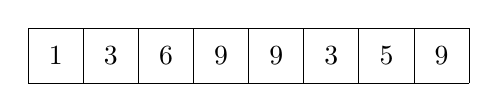
\begin{tikzpicture}[scale=0.7]
\draw (0,0) grid (8,1);
\node at (0.5,0.5) {$1$};
\node at (1.5,0.5) {$3$};
\node at (2.5,0.5) {$6$};
\node at (3.5,0.5) {$9$};
\node at (4.5,0.5) {$9$};
\node at (5.5,0.5) {$3$};
\node at (6.5,0.5) {$5$};
\node at (7.5,0.5) {$9$};
\end{tikzpicture}
\end{center}
li correspon el seg\"uent vector de comptatge:
\begin{center}
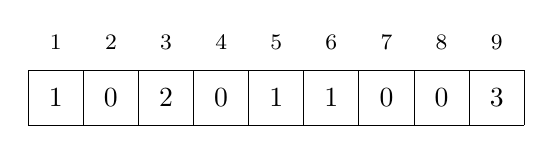
\begin{tikzpicture}[scale=0.7]
\draw (0,0) grid (9,1);
\node at (0.5,0.5) {$1$};
\node at (1.5,0.5) {$0$};
\node at (2.5,0.5) {$2$};
\node at (3.5,0.5) {$0$};
\node at (4.5,0.5) {$1$};
\node at (5.5,0.5) {$1$};
\node at (6.5,0.5) {$0$};
\node at (7.5,0.5) {$0$};
\node at (8.5,0.5) {$3$};

\footnotesize

\node at (0.5,1.5) {$1$};
\node at (1.5,1.5) {$2$};
\node at (2.5,1.5) {$3$};
\node at (3.5,1.5) {$4$};
\node at (4.5,1.5) {$5$};
\node at (5.5,1.5) {$6$};
\node at (6.5,1.5) {$7$};
\node at (7.5,1.5) {$8$};
\node at (8.5,1.5) {$9$};
\end{tikzpicture}
\end{center}

Per exemple, el valor a la posició 3
del vector de comptatge és 2,
perquè l'element 3 apareix 2 vegades
al vector original.

La construcció del vector de comptatge
triga temps $O(n)$. Després d'això, el vector ordenat
es crea en temps $O(n)$ perquè recuperem el nombre
d'ocurrències de cada element en el vector de comptatge.
Per tant, la complexitat temporal total és $O(n)$.

L'ordenació per comptatge és un algorisme molt eficient
però només es pot fer servir quan el valor $c$
és prou petit, ja que en cas contrari no podem fer servir els
elements del vector com a índexs del vector de comptatge.

\section{Ordenació en C++}

\index{ordenar@\texttt{ordenar}}

Gairebé mai és bona idea fer servir
algorismes d'ordenació casolans
en un concurs, perquè els llenguatges de programació
ja venen amb molt bones implementacions.
Per exemple, la biblioteca estàndard de C++ conté
la funció \texttt{sort} que es pot fer servir per a ordenar
vectors i altres estructures de dades.

Hi ha molts avantatges en fer servir les funcions de les biblioteques.
Primer, estalvia temps perquè no cal implementar la funció.
Segon, la implementació de la biblioteca és
certament correcta i eficient: no és probable
que la teva funció de classificació casolana sigui millor.

En aquesta secció veurem com fer servir la
funció C++ \texttt{sort}.
El codi següent ordena
un vector en ordre creixent:
\begin{lstlisting}
vector<int> v = {4,2,5,3,5,8,3};
sort(v.begin(),v.end());
\end{lstlisting}
Després de l'ordenació, el contingut del
vector és
$[2,3,3,4,5,5,8]$.
Els elements s'ordenen per defecte en ordre creixent,
però també és possible ordenar-los en ordre invers:
\begin{lstlisting}
sort(v.rbegin(),v.rend());
\end{lstlisting}
També és possible ordenar un array ordinari de C:
\begin{lstlisting}
int n = 7; // mida del array
int a[] = {4,2,5,3,5,8,3};
sort(a,a+n);
\end{lstlisting}

El codi següent ordena la cadena \texttt{s}:
\begin{lstlisting}
string s = "monkey";
sort(s.begin(), s.end());
\end{lstlisting}
Ordenar una cadena significa que ordenem tots
els seus caràcters.
Per exemple, la cadena ``monkey'' es converteix en ``ekmnoy''.

\subsubsection{Operadors de comparació}

\index{operador de comparació}

La funció \texttt{sort} requereix
que es defineix un \key{operador de comparació} per al tipus de dades
dels elements a ordenar.
Quan ordenem, es farà servir aquest operador
sempre que sigui necessari esbrinar l'ordre de dos elements.

La majoria dels tipus de dades C++ tenen un operador de comparació definit
per defecte, i els elements d'aquests tipus es poden ordenar automàticament.
Per exemple, els nombres s'ordenen segons els seus valors i
les cadenes estan ordenades per ordre alfabètic.

\index{parell@\texttt{pair}}

Els parells (\texttt{pair}) s'ordenen en funció dels seus
primers elements (\texttt{first}).
Si els primers elements dels dos parells són iguals,
aleshores s'ordenen segons els segons elements (\texttt{second}):
\begin{lstlisting}
vector<pair<int,int>> v;
v.push_back({1,5});
v.push_back({2,3});
v.push_back({1,2});
sort(v.begin(), v.end());
\end{lstlisting}
Després d'això, l'ordre de les parelles és
$(1,2)$, $(1,5)$ i $(2,3)$.

\index{tupla@\texttt{tuple}}

De manera semblant, les tuples (\texttt{tuple})
s'ordenen pel primer element,
seguit pel segon element en cas d'empat, el tercer, etc.\footnote{
Tingueu en compte que en alguns compiladors antics,
és necessari fer servir la funció \texttt{make\_tuple} en lloc de les
claus (per exemple, \texttt{make\_tuple(2,1,4)} en lloc de \texttt{\{2,1,4\}}).}:
\begin{lstlisting}
vector<tuple<int,int,int>> v;
v.push_back({2,1,4});
v.push_back({1,5,3});
v.push_back({2,1,3});
sort(v.begin(), v.end());
\end{lstlisting}
Després d'això, l'ordre de les tuples és
$(1,5,3)$, $(2,1,3)$ i $(2,1,4)$.

Aquesta idea de les tuples també s'estén als vectors.

\subsubsection{Estructures definides per l'usuari}

Les estructures definides per l'usuari no tenen un
operador de comparació
definit per defecte.
Una manera de fer-ho és definir l'operador
a dintre de la estructura de dades com a funció
\texttt{operator<},
el paràmetre del qual és un altre element del mateix tipus.
L'operador hauria de retornar \texttt{true}
si l'element és més petit que el paràmetre,
i \texttt{false} en cas contrari.

Per exemple, l'estructura \texttt{P} següent
conté les coordenades $x$ i $y$ d'un punt.
L'operador de comparació es defineix de manera que
els punts s'ordenen per la coordenada $x$
i, en cas d'empat, per la coordenada y.

\begin{lstlisting}
struct P {
    int x, y;
    operador bool<(const P &p) {
        if (x != p.x) return x < p.x;
        else return y < p.y;
    }
};
\end{lstlisting}

\subsubsection{Funcions de comparació}

\index{funció de comparació}

També és possible donar una
\key{funció de comparació} externa (\texttt{callback}) a la funció
\texttt{sort}. 
Per exemple, la següent funció de comparació \texttt{comp}
ordena les cadenes primer per longitud i segon per ordre alfabètic:

\begin{lstlisting}
bool comp(const string& a, const string& b) {
    if (a.size() != b.size()) return a.size() < b.size();
    return a < b;
}
\end{lstlisting}
Ara podem ordenar un vector de cadenes així:
\begin{lstlisting}
sort(v.begin(), v.end(), comp);
\end{lstlisting}

N. del T.: També podem fer servir expressions lambda:
\begin{lstlisting}
sort(v.begin(), v.end(), [](const string& a, const string& b) {
    return (a.size() != b.size()) ? (a.size() < b.size()) : (a < b);
});
\end{lstlisting}

\section{Cerca binària}

\index{cerca binària}

Un mètode general per cercar un element
en un vector és fer servir un bucle \texttt{for}
que iteri els elements del vector.
Per exemple, el codi següent cerca
un element $x$ en el vector $v$:

\begin{lstlisting}
for (int i = 0; i < n; i++) {
    if (v[i] == x) {
        // trobem x a la posicio i
    }
}
\end{lstlisting}

La complexitat temporal d'aquest codi és $O(n)$,
perquè en el pitjor dels casos, cal comprovar
tots els elements del vector.
Si l'ordre dels elements és arbitrari,
aquesta és també la millor solució, perquè
no tenim informació addicional per saber en quin
lloc del vector hem de cercar l'element $x$.

Tanmateix, si el vector està \emph{ordenat},
la situació és diferent.
En aquest cas és possible realitzar el
cerca molt més ràpid, perquè l'ordre dels
elements del vector guia la cerca.
El següent algorisme de \key{cerca binària}
cerca eficientment un element en un vector ordenat
en temps $O(\log n)$.

\subsubsection{Mètode 1}

La forma habitual d'implementar la cerca binària
s'assembla a buscar una paraula en un diccionari.
La cerca manté una regió activa al vector,
que inicialment conté tots els elements del vector.
Aleshores, es fa una sèrie de passos,
cadascun dels quals redueix a la meitat la mida de la regió
activa.

A cada pas, la cerca comprova l'element central
de la regió activa.
Si l'element central és l'element objectiu,
la cerca acaba.
En cas contrari, la cerca continua de forma recursiva
a la meitat esquerra o dreta de la regió,
en funció del valor de l'element mitjà.

La idea anterior es pot implementar de la següent manera:
\begin{lstlisting}
int a = 0, b = n-1;
while (a <= b) {
    int k = (a+b)/2;
    if (v[k] == x) {
        // trobem x a la posicio k
    }
    if (v[k] > x) b = k-1;
    else a = k+1;
}
\end{lstlisting}

En aquesta implementació, la regió activa és $a \ldots b$,
i la regió inicial és $0 \ldots n-1$.
L'algorisme redueix a la meitat la mida de la regió a cada pas,
per tant, la complexitat temporal és $O(\log n)$.

\subsubsection{Mètode 2}

Un mètode alternatiu per implementar la cerca binària
es basa en una manera eficient d'iterar
els elements del vector.
La idea és fer salts i reduir la velocitat
quan ens acostem a l'element objectiu.

La cerca passa per el vector d'esquerra a
dreta, i la longitud inicial del salt és $n/2$.
A cada pas, la longitud del salt es reduirà a la meitat:
primer $n/4$, després $n/8$, $n/16$, etc., fins que
finalment la longitud és 1.
Després dels salts, l'element objectiu o bé
s'ha trobat o bé sabem que no apareix al vector.

El codi següent implementa la idea anterior:
\begin{lstlisting}
int k = 0;
for (int b = n/2; b >= 1; b /= 2) {
    while (k+b < n && v[k+b] <= x) k += b;
}
if (v[k] == x) {
    // trobem x a la posicio x
}
\end{lstlisting}

Durant la cerca, la variable $b$
conté la longitud actual del salt.
La complexitat temporal és també $O(\log n)$,
perquè el codi del bucle \texttt{while}
es realitza com a màxim dues vegades per a cada llargada de salt.

\subsubsection{Funcions C++}

La biblioteca estàndard de C++ conté les funcions següents
que es basen en cerca binària i triguen temps logarítmic:

\begin{itemize}
\item \texttt{lower\_bound} retorna un punter al
primer element del vector el valor del qual és almenys $x$.
\item \texttt{upper\_bound} retorna un punter a
primer element del vector el valor del qual és més gran que $x$.
\item \texttt{equal\_range} retorna els dos punters anteriors.
\end{itemize}

Les funcions assumeixen que el vector està ordenat.
Si aquest primer element no existeix, les funcions retornen un
punter a una posició més enllà de l'últim element del vector\footnote{
N. del T.: Dit d'altra manera: l'interval semi-obert
[\texttt{lower\_bound(x)},\texttt{upper\_bound(x)})
  assenyala en quin lloc són, o haurien de ser, els elements amb
  valor $x$.}.
Per exemple, el codi següent esbrina si
un vector ordenat conté un element amb el valor $x$:

\begin{lstlisting}
int k = lower_bound(v.begin(),v.end(),x) - v.begin();
if (k < n && v[k] == x) {
    // trobem x a la posicio k
}
\end{lstlisting}

El codi següent compta el nombre d'elements
amb valor $x$:

\begin{lstlisting}
auto a = lower_bound(v.begin(), v.end(), x);
auto b = upper_bound(v.begin(), v.end(), x);
cout << b-a << "\n";
\end{lstlisting}

Utilitzant \texttt{equal\_range}, el codi queda més curt:

\begin{lstlisting}
auto r = equal_range(v.begin(), v.end(), x);
cout << r.second-r.first << "\n";
\end{lstlisting}

\subsubsection{Trobar la solució més petita}

Un ús important de la cerca binària és
trobar la posició on canvia el valor d'una \emph{funció}.
Suposem que volem trobar el valor més petit $k$
que és una solució vàlida per a un problema.
Ens donen una funció $\texttt{ok}(x)$
que retorna \texttt{true} si $x$ és vàlida
i \texttt{false} en cas contrari.
A més, sabem que $\texttt{ok}(x)$ és \texttt{false}
quan $x<k$ i \texttt{true} quan $x \ge k$.
És a dir:

\begin{center}
\begin{tabular}{r|rrrrrrrr}
$x$ & 0 & 1 & $\cdots$ & $k-1$ & $k$ & $k+1$ & $\cdots$ \\
\hline
$\texttt{ok}(x)$ & \texttt{f} & \texttt{f}
& $\cdots$ & \texttt{f} & \texttt{t} & \texttt{t} & $\cdots$ \\
\end{tabular}
\end{center}

\noindent
Ara, el valor de $k$ es pot trobar mitjançant la cerca binària:

\begin{lstlisting}
int x = -1;
for (int b = z; b >= 1; b /= 2) {
    while (!ok(x+b)) x += b;
}
int k = x+1;
\end{lstlisting}
<
La cerca troba el valor més gran de $x$ per al qual
$\texttt{ok}(x)$ és \texttt{false}.
Així, el següent valor $k=x+1$
és necessàriament el valor més petit possible per al qual
$\texttt{ok}(k)$ és \texttt{true}.
La longitud inicial del salt $z$ ha de ser
prou gran, per exemple algun valor
per al qual sabem per endavant que $\texttt{ok}(z)$ és \texttt{true}.

L'algorisme crida a la funció \texttt{ok}
$O(\log z)$ vegades, per tant la complexitat total
depèn de la funció \texttt{ok}.
Per exemple, si aquesta funció triga temps $O(n)$,
la complexitat total és $O(n \log z)$.

\subsubsection{Trobar el valor màxim}

La cerca binària també es pot fer servir per trobar
el valor màxim d'una funció que primer creix i després
decreix.
La nostra tasca és trobar una posició $k$ tal que

\begin{itemize}
\item
$f(x)<f(x+1)$ quan $x<k$, i
\item
$f(x)>f(x+1)$ quan $x \ge k$.
\end{itemize}

La idea és fer servir la cerca binària
per trobar el valor més gran de $x$
tal que $f(x)<f(x+1)$.
Això implica que $k=x+1$
perquè $f(x+1)>f(x+2)$.
El codi següent implementa la cerca:

\begin{lstlisting}
int x = -1;
for (int b = z; b >= 1; b /= 2) {
    while (f(x+b) < f(x+b+1)) x += b;
}
int k = x+1;
\end{lstlisting}

Tingueu en compte que, a diferència de la cerca binària ordinària,
en aquest cas no permetem que els valors consecutius
de la funció siguin iguals, donat que no sabríem
en quina direcció continuar la cerca.
